\section{AG3: one complete correction and its passive comparison\workstar}
The second investigation of the homogeneous goal applies a domain-preserving correction to the \emph{complete} actual AG2 mixing family. Its bound is
\begin{equation}
 \norm{R'}_{3/2}\le\gamma\norm B_2,
 \qquad
 \gamma=\begin{cases}3060/3623,&0\le M\le10^{-3},\\
 5949/96812,&0\le M\le10^{-4}.
 \end{cases}
 \label{eq:ag3-headline}
\end{equation}
This compares different support weights. The main coefficient is weaker than the passive bound obtained by leaving $B$ unchanged and measuring it at weight $3/2$. The narrow coefficient improves that universal upper ceiling, but neither interval proves improvement over the actual old lower-weight norm. The exact full conjugation, domains, retained diagonal and scalar terms are substantive parts of the accepted result.

\subsection{A bare-reference inverse for every generated support}
The actual input from AG2 is
\begin{equation}
 H_{\rm in}=C_\Lambda I+H_0+D_{\rm next}+B,\qquad
 D_{\rm next}=D+Z,\quad r=\norm B_2,\quad d=\norm{D_{\rm next}}_2.
 \label{eq:ag3-input}
\end{equation}
Every assigned connected support $Y$ has at least four coarse blocks, with no uniform upper size. All original and transported histories remain indexed. Coincident supports are not canceled or assigned smaller supports to alter $r$. With the admitted cap $K$ from AG2,
\begin{equation}
 r\le K,\qquad d\le64M+2K,\qquad
 \abs{\langle\psi,D_{\rm next}\psi\rangle}
 \le(4M+K/8)\langle\psi,H_0\psi\rangle.
 \label{eq:ag3-input-budgets}
\end{equation}
Here $K=7/1000$ or $7/100000$ on the main or narrow interval, respectively. The actual norm $r$ is distinct from this upper cap and from an extensive operator norm.

Since $B_Y=P_YK_YQ_Y+Q_YK_YP_Y$, write $v_Y=B_Y\Omega_Y$ and define a new generator $T$ (called $X$ in the AG3 reports):
\begin{equation}
 u_Y=(H_{0,Y}|_{Q_Y})^{-1}v_Y,\qquad
 T_Y=|u_Y\rangle\langle\Omega_Y|-|\Omega_Y\rangle\langle u_Y|,
 \qquad T=\sum_Y T_Y.
 \label{eq:ag3-generator}
\end{equation}
The reduced local reference is at least one. Spectral calculus gives $u_Y\in D(H_{0,Y})$, $H_{0,Y}u_Y=v_Y$, and $\norm{T_Y}\le\norm{B_Y}$. The local products have bounded extensions and $[T_Y,H_{0,Y}]=-B_Y$ on the domain. Extend by the exterior identity. Commuting nonnegative local and exterior energies give $D(H_0)=D(H_{0,Y})\cap D(H_{0,\rm ext})$, so the full domain is preserved. This is not regularization of an arbitrary exterior vector and is not the operator obtained with a global vacuum projector.

In each finite cuboid,
\begin{equation}
 \sum_Y\norm{B_Y}\le |\Lambda|r/64,\qquad
 \sum_Y\norm{T_Y}\le |\Lambda|r/64,\qquad \norm T_2\le r.
\end{equation}
Closedness of $H_0$ and convergence of the bounded commutators give $[T,H_0]=-B$. The relation $H_0T\psi=TH_0\psi+B\psi$ supplies the graph-norm bound; both exponentials preserve $D(H_0)$. No bounded infinite-volume global generator or unitary is asserted. This inverse uses $H_0$ alone, so the changed diagonal is retained as a commutator defect.

\subsection{The full infinite remainder with an actual denominator}
First integrate the established bounded commutator on $D(H_0)$, then expand only bounded conjugations. The exact result is
\begin{align}
 e^T H_{\rm in}e^{-T}&=C_\Lambda I+H_0+D_{\rm next}+R',\notag\\
 R'&=\sum_{n\ge1}\left(
 \frac{\ad_T^n D_{\rm next}}{n!}
 +\frac{n\ad_T^n B}{(n+1)!}\right).
 \label{eq:ag3-full-tail}
\end{align}
In particular $[T,D_{\rm next}]+[T,B]/2$ remains at first order; the old scalar commutes but stays in the Hamiltonian. This does not assume a norm-convergent BCH series for unbounded $H_0$.

For indexed interactions $U,V$ and $a>b\ge3/2$, nonempty intersection yields $b^{|Y\cup Z|}\le b^{|Y|}b^{|Z|}/b$. Retaining both root placements and using $m\exp[-m\log(a/b)]\le1/(e\log(a/b))$ proves
\begin{equation}
 \norm{[U,V]}_b\le\frac{4}{be\log(a/b)}\norm U_a\norm V_a.
 \label{eq:ag3-commutator}
\end{equation}
Every repeated index and complete union is included. The proof imposes no maximum support size and establishes the new output-weight range directly.

At nested order $n$, allocate $\ell/n$ per bracket with $\ell=\log(4/3)$. All intermediate weights are at least $3/2$. The elementary bound $n!\ge(n/e)^n$ gives
\begin{equation}
 \frac{\norm{\ad_T^n V}_{3/2}}{n!}
 \le(\bar c r)^n\norm V_2,
 \qquad \bar c=\frac{288}{31}.
 \label{eq:ag3-nested}
\end{equation}
Indeed $\ell\ge31/108$ follows by integrating
$1/(1+t)=1-t+t^2-t^3+t^4/(1+t)$ on $[0,1/3]$; its remainder is positive. Therefore $(8/3)/\ell\le\bar c$. With $\theta=\bar c r<1$, the complete positive tail yields
\begin{equation}
 \norm{R'}_{3/2}\le r\,\frac{\bar c(d+r)}{1-\bar c r},
 \qquad
 \text{tail after order }N\le(d+r)\frac{\theta^{N+1}}{1-\theta}.
 \label{eq:ag3-ratio}
\end{equation}
Only the increasing coefficient uses $r\le K$ and $d\le64M+2K$; the actual $r$ remains outside. At the main and narrow endpoints $\theta\le252/3875$ and $63/96875$, respectively. These positive monotonicities establish continuous-interval coverage and give \eqref{eq:ag3-headline}. If $r=0$, each indexed $B_Y$ vanishes, $T=0$ and $R'=0$, without division; both coupling signs are covered by $M=7|\tau|$.

\subsection{What passive reweighting already provides}
Minimum support size four gives, for the \emph{same} indexed input family,
\begin{equation}
 \norm B_{3/2}\le(3/4)^4\norm B_2=\frac{81}{256}r.
 \label{eq:ag3-passive}
\end{equation}
Exact comparison places $3060/3623$ above this ceiling and $5949/96812$ below it. The main active certificate consequently does not certify a benefit over doing no correction at the lower weight. The narrow active certificate is smaller than the universal passive upper ceiling, but two upper bounds do not compare the actual norms. A diagnostic family concentrated on one support of size $m$ has passive ratio $(3/4)^m$, arbitrarily small as $m$ grows. This is a counterexample to the proposed general inference, not an evaluation of the actual AG2 trajectory.

\begin{figure}[htbp]
 \centering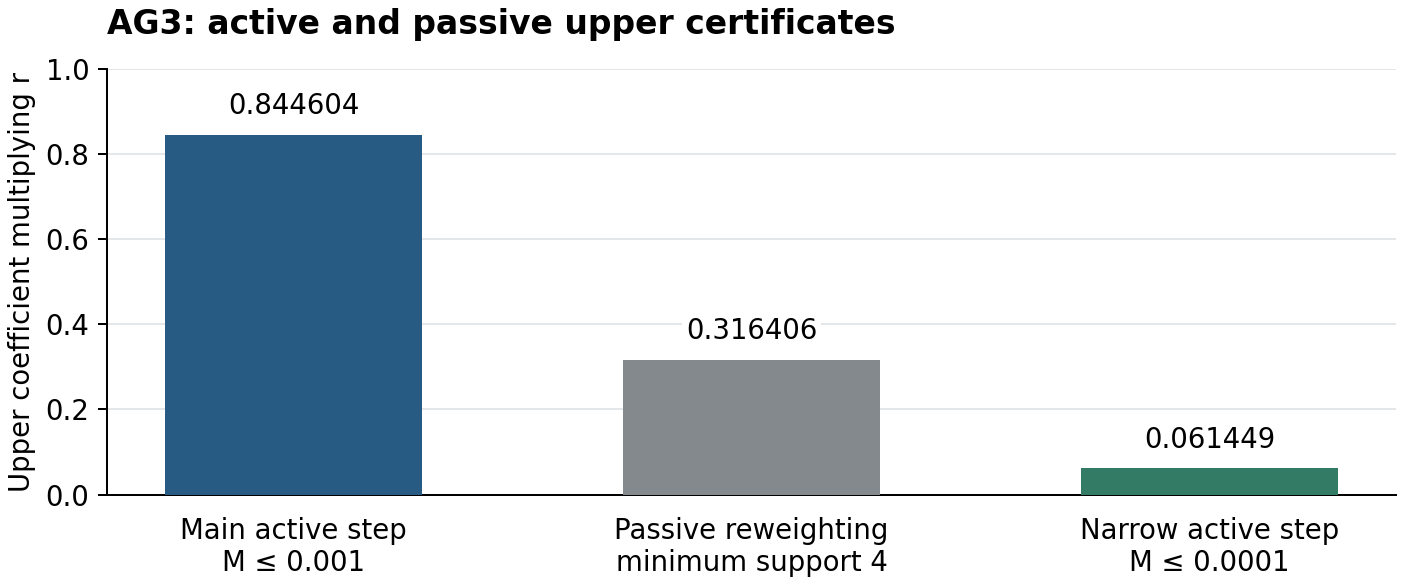
\includegraphics[width=.94\linewidth]{figures/ag3-passive-comparison.png}
 \caption{Sufficient coefficients multiplying the same actual $r=\norm B_2$. Active bars bound the complete corrected $\norm{R'}_{3/2}$; the passive bar bounds the unchanged $\norm B_{3/2}$. All values are exact rational certificates rendered as decimals. They do not evaluate either actual lower-weight norm, establish same-weight contraction, or measure theorem completion.}
 \label{fig:ag3-passive}
\end{figure}

\subsection{Retained scalars, diagonals and the reference-only gap}
Split every generated self-adjoint indexed residual $J_Y$ on its full support:
\begin{align}
 c'_Y&=\langle\Omega_Y,J_Y\Omega_Y\rangle,\qquad
 B'_Y=P_YJ_YQ_Y+Q_YJ_YP_Y,\notag\\
 Z'_Y&=Q_Y(J_Y-c'_YI)Q_Y,
 \qquad J_Y=c'_YI+B'_Y+Z'_Y.
\end{align}
The respective norm costs are one, one and two. Put $W=\gamma K$ and $C'=\sum_Yc'_Y$. Retaining the old scalar and minimum assigned support gives
\begin{align}
 \norm{B'}_{3/2}&\le\gamma r\le W,\qquad
 \norm{Z'}_{3/2}\le2W,\notag\\
 \frac{|C_\Lambda+C'|}{|\Lambda|}&\le\frac K{64}+\frac{4W}{81},\qquad
 |\langle\psi,Z'\psi\rangle|\le\frac{32W}{81}\langle\psi,H_0\psi\rangle.
 \label{eq:ag3-scalar-diagonal}
\end{align}
The extracted centered reference $G'=H_0+D_{\rm next}+Z'$ has domain $D(H_0)$, annihilates the product vacuum, and satisfies
\begin{equation}
 G'\ge\left(1-4M-\frac K8-\frac{32W}{81}\right)H_0.
 \label{eq:ag3-reference}
\end{equation}
The exact endpoint coefficient is $258975047/260856000>124/125$ on the main interval and $174190074443/174261600000>1999/2000$ on the narrow interval. These are normalized \emph{reference-only} gap floors. Physical reference energies multiply the unchanged $\delta=\alpha/8$. The full corrected operator remains $(C_\Lambda+C')I+G'+B'$. Its mixing is not discarded, its scalar is not identified with the true interacting ground energy, and its gap is unproved.

The reverse derivation additionally applies passive reweighting to the carried diagonal, obtaining $\norm{D_{\rm next}+Z'}_{3/2}\le(81/256)d+2W$. The forward and skeptical bound $d+2W$ is also valid. This difference in sufficient estimates is preserved rather than silently merged.

The bare-inverse strategy originated in the Newton post-AG2 review; the advisor's overlap refinement and proposed constant were shared before the contract. The directions independently derived and implemented the frozen target, not independently invented its premise. The skeptic's independent production preceded exchange; its additional passive interpretation and the reverse supplemental note were post-freeze reviews. Exact finite-matrix, exterior-domain, complete-support and denominator controls test the stated algebra and inference. They are not physical SU(2) cutoff simulations or observations.

Both the previous $9/4\to2$ and current $2\to3/2$ margins are spent. Growing-support controls reject a free return to weight two, and a generic fixed-weight commutator control rejects a universal bilinear constant for that broad class. No all-stage conclusion or repair of the earlier O2 majorant follows. A future iteration requires its own remaining weight schedule, retained-diagonal estimates and convergence theorem. This loop proves no full homogeneous gap, physical scale matching or four-dimensional continuum construction.
